% \documentclass{lab-report}
% \usepackage{mathpazo} % Fonte MathPazo
% \usepackage{times} % Fonte Times New Roman
% \usepackage{helvet} % Fonte Helvetica
% \renewcommand{\familydefault}{\sfdefault}

% \usepackage{karnaugh-map}
% \usepackage{csvsimple}
% \usepackage{tabularray}

\documentclass[a4,12pt]{horizon-theme}
\usepackage{lipsum}
\usepackage{fontawesome5}
\usepackage{graphicx,url}
\usepackage{float}
\usepackage{amsmath}
\usepackage{booktabs}
\usepackage{makecell}
\usepackage{array}
\usepackage{multirow}
\usepackage{caption}
\usepackage{subcaption}
\usepackage{siunitx}
\usepackage{enumerate}
\usepackage{gensymb}
\usepackage{csvsimple}
% \usepackage{tabularray}
\usepackage{stackengine}
\usepackage{xcolor, colortbl}
% \usepackage[round]{natbib}
\usepackage{karnaugh-map}
\usepackage{stackengine}
% \usepackage{longtable}
% \usepackage{minted}
\usepackage{fontawesome}

\strutlongstacks{T}


%%%%%%%%%%%%%%%%%%%%%%%%%%%%%%%%%%%%%%%
% Início: informações da capa
%%%%%%%%%%%%%%%%%%%%%%%%%%%%%%%%%%%%%%%
% ~~> Mudar abaixo a cada experimento <~~
% \setExpNumber{3}
% \setExpTitle{Decodificadores e Multiplexadores}
% \setDate{04/04/2022}
% Não precisa mudar abixo
% \setTeacher{Glauber de Bona}
% \setBancada{B3}
% \setTurma{10}
% \setMemberOne{Natanael Magalhães Cardoso}{8914122}
% \setMemberTwo{Renato Naves Fleury}{11805269}
%%%%%%%%%%%%%%%%%%%%%%%%%%%%%%%%%%%%%%%%
% Fim: informações da capa
%%%%%%%%%%%%%%%%%%%%%%%%%%%%%%%%%%%%%%%%

% Cover Config
% \configCover{<num. do exp.>}{<data>}{<título>}
\configCover{3}{29/03/2022}{Decodificadores e Multiplexadores}

% \newcommand{\n}[1]{\overline{#1}}


\begin{filecontents*}{tb_verdade.csv}
A3,A2,A1,A0,Y
0,0,0,0,0
0,0,0,1,0
0,0,1,0,0
0,0,1,1,1
0,1,0,0,0
0,1,0,1,0
0,1,1,0,1
0,1,1,1,1
1,0,0,0,0
1,0,0,1,1
1,0,1,0,0
1,0,1,1,1
1,1,0,0,0
1,1,0,1,0
1,1,1,0,0
1,1,1,1,0
\end{filecontents*}

\begin{filecontents*}{tb_verdade_dec_debug.csv}
A3,A2,A1,A0,O0,O1,O2,O3,O4,O5,O6,O7,O8,O9,O10,O11,O12,O13,O14,O15,Y
0,0,0,0,0,1,1,1,1,1,1,1,1,1,1,1,1,1,1,1,0
0,0,0,1,1,0,1,1,1,1,1,1,1,1,1,1,1,1,1,1,0
0,0,1,0,1,1,0,1,1,1,1,1,1,1,1,1,1,1,1,1,0
0,0,1,1,1,1,1,0,1,1,1,1,1,1,1,1,1,1,1,1,1
0,1,0,0,1,1,1,1,0,1,1,1,1,1,1,1,1,1,1,1,0
0,1,0,1,1,1,1,1,1,0,1,1,1,1,1,1,1,1,1,1,0
0,1,1,0,1,1,1,1,1,1,0,1,1,1,1,1,1,1,1,1,1
0,1,1,1,1,1,1,1,1,1,1,0,1,1,1,1,1,1,1,1,1
1,0,0,0,1,1,1,1,1,1,1,1,0,1,1,1,1,1,1,1,0
1,0,0,1,1,1,1,1,1,1,1,1,1,0,1,1,1,1,1,1,1
1,0,1,0,1,1,1,1,1,1,1,1,1,1,0,1,1,1,1,1,0
1,0,1,1,1,1,1,1,1,1,1,1,1,1,1,0,1,1,1,1,1
1,1,0,0,1,1,1,1,1,1,1,1,1,1,1,1,0,1,1,1,0
1,1,0,1,1,1,1,1,1,1,1,1,1,1,1,1,1,0,1,1,0
1,1,1,0,1,1,1,1,1,1,1,1,1,1,1,1,1,1,0,1,0
1,1,1,1,1,1,1,1,1,1,1,1,1,1,1,1,1,1,1,0,0
\end{filecontents*}

\begin{filecontents*}{tb_verdade_mux_debug.csv}
A3,A2,A1,A0,O0,O1,Y
0,0,0,0,0,0,0
0,0,0,1,0,0,0
0,0,1,0,0,0,0
0,0,1,1,1,0,1
0,1,0,0,0,0,0
0,1,0,1,0,0,0
0,1,1,0,1,0,1
0,1,1,1,1,0,1
1,0,0,0,0,0,0
1,0,0,1,0,1,1
1,0,1,0,0,0,0
1,0,1,1,0,1,1
1,1,0,0,0,0,0
1,1,0,1,0,0,0
1,1,1,0,0,0,0
1,1,1,1,0,0,0
\end{filecontents*}


\begin{filecontents*}{tb_verdade_exp.csv}
A3,A2,A1,A0,Y_sim,Y_exp_dec,Y_exp_mux
0,0,0,0,0,0,0
0,0,0,1,0,0,0
0,0,1,0,0,0,0
0,0,1,1,1,1,1
0,1,0,0,0,0,0
0,1,0,1,0,0,0
0,1,1,0,1,1,1
0,1,1,1,1,1,1
1,0,0,0,0,0,0
1,0,0,1,1,1,1
1,0,1,0,0,0,0
1,0,1,1,1,1,1
1,1,0,0,0,0,0
1,1,0,1,0,0,0
1,1,1,0,0,0,0
1,1,1,1,0,0,0
\end{filecontents*}






\begin{document}
\horizonCover

\horizonTitle

\section{Introdução} % R
À medida que a complexidade dos ciruitos digitais aumenta, CIs simples, como os do tipo SSI (Small Scale Integration), vão se tornando inviáveis de serem utilizados, por possuírem poucas portas lógicas acabam deixando o projeto mais caro e menos compacto. Uma alternativa para esse problema é a utilização de circuitos decodificadores e multiplexadores \cite{saraiva}.

Um decodificador é um dispositivo que recebe $n$ entradas e produz $2^n$ saídas. A saída tera valor ``1'' apenas no índice que representa o valor de entrada em decimal.

Já um multiplexador possui $2^n$ entradas de dados (numeradas de 0 à $2^n-1$), $n$ entradas de seleção e uma saída. A saída é ligada à entrada que corresponde ao valor das entradas de seleção em decimal.





\section{Objetivos} % N
O objetivo deste projeto é explorar a técnica de síntese de dois circuitos digitais a partir de uma Tabela Verdade fornecida (Tabela \ref{tab:tabela_verdade}) usando decodificadores 74138 TTL para um e multiplexadores 74151 TTL para outro, contemplando as etapas de criação do diagrama de blocos, simulação, montagem e testes.





\section{Planejamento} % N, R
\label{sec:plan}

Neste planejamento estão descritos dois circuitos digitais, um construído com decodificador (Seção \ref{sec:dec}) e outro com multiplexador (Seção \ref{sec:mux}). Ambos os circuitos possuem a mesma Tabela Verdade, descrita na Tabela \ref{tab:tabela_verdade}. Os circuitos foram projetados para funcionarem separadamente. A Figura \ref{fig:diagrama_blocos} mostra o diagrama de blocos para ambos os circuitos, onde A3, A2, A1 e A0 são os sinais de entrada e Y o sinal de saída.

\begin{figure}[!ht]
  \centering
  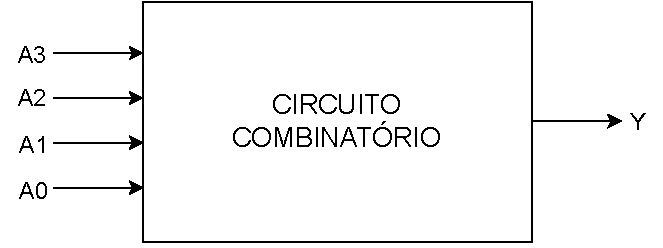
\includegraphics[width=0.7\textwidth]{diagrama_blocos.pdf}
  \caption{Diagrama de blocos para ambos os circuitos}
  \label{fig:diagrama_blocos}
\end{figure}

\begin{table}[!ht]
  \centering
  \caption{Tabela Verdade dos circuitos construídos com decodificadores e multiplexadores apresentando o valor da saída $Y$ com entradas $A_3A_2A_1A_0$}
  \label{tab:tabela_verdade}
  \doubleRuleSep
  \begin{tabular}{rrrrr}
    \doubleTopRule
    $A_3$     & $A_2$     & $A_1$      & $A_0$     & $Y$       \\
    \midrule
    \csvreader[head to column names, late after line=\\]{tb_verdade.csv}{}%
    {\csvcoli & \csvcolii & \csvcoliii & \csvcoliv & \csvcolv} %
    \doubleBottomRule
  \end{tabular}
\end{table}



\newpage
\subsection{Circuito com Decodificador} % N
\label{sec:dec}

\subsubsection{Diagrama lógico do circuito}
\label{sec:dec_diagrama}

A partir da Tabela \ref{tab:tabela_verdade}, foi projeto um circuito digital mostrado no Diagrama Lógico da Fig. \ref{fig:dec_diagrama} usando dois decodificadores 74138, identificados por C1 e C2. As informações das entradas Vcc e Gnd dos componentes utilizados estão na Tabela \ref{tab:dec_entradas}.

O bit de entrada mais significativo foi conectado na porta enable do decodificador C1 e invertido na porta enable do decodificador C2. Com isso, conseguimos a decodificação do sinal de entrada de 4 bits a partir do cascateamento de dois decodificadores 3x8, gerando um decodificador 4x16 \cite{saraiva}. Com o decodificador criado, selecionamos os sinais com ``1'' na Tabela \ref{tab:tabela_verdade} e usamos como entrada de uma operação NAND (C4, C5 e C6) para obter o valor de $Y$.

\begin{figure}[!ht]
  \centering
  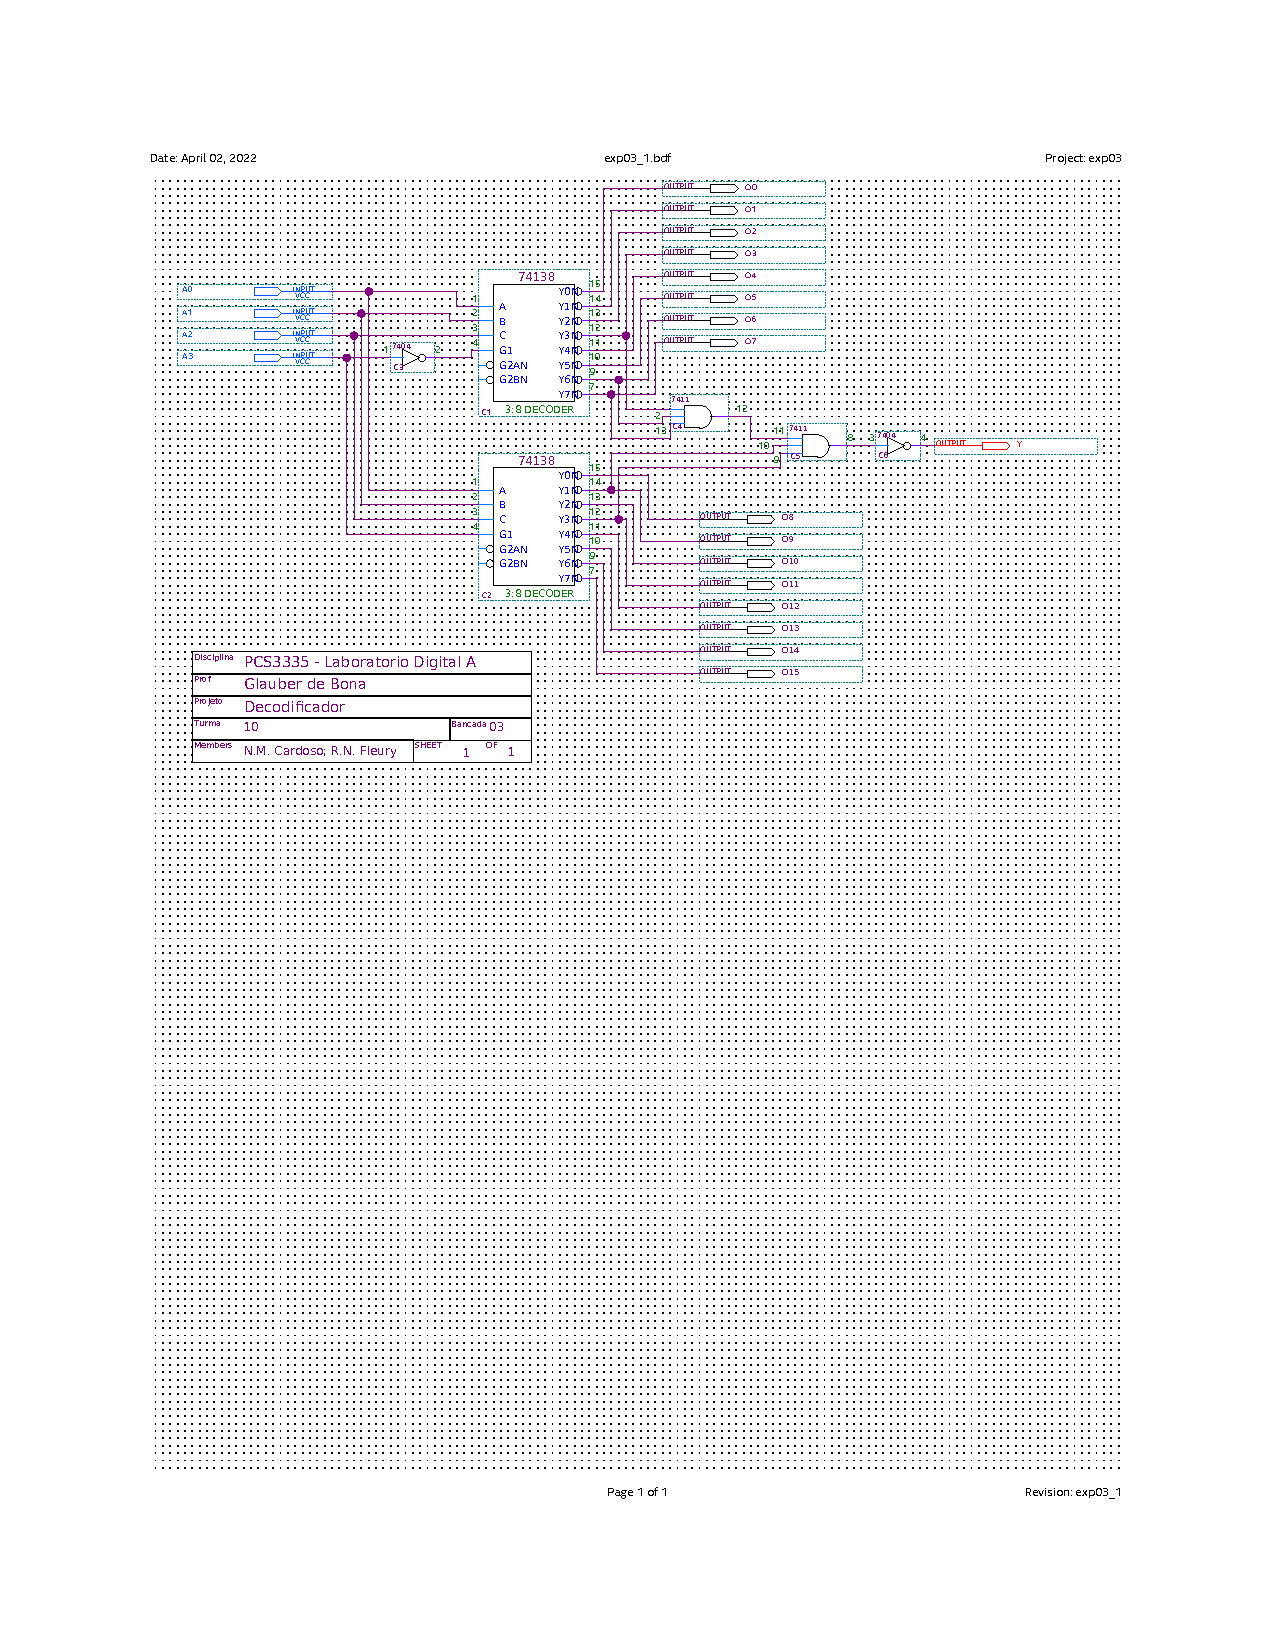
\includegraphics[width=\textwidth, trim={30mm, 150mm, 30mm, 30mm}, clip]{diagrama_decoder.pdf}
  \caption[]{Diagrama lógico\footnotemark do circuito criado a partir da Tabela \ref{tab:tabela_verdade} com o uso de dois decodificadores 74138 TTL.}
  \label{fig:dec_diagrama}
\end{figure}
\footnotetext{Imagem vetorial, é possível ampliar sem perder qualidade}


\begin{table}[!ht]
  \centering
  \caption{Informação das entradas Vcc e Gnd para cada componente identificado na Fig. \ref{fig:dec_diagrama}}
  \label{tab:dec_entradas}
  \doubleRuleSep
  \begin{tabular}{lrrr}
    \doubleTopRule
    Posição & Comp. & Vcc & Gnd \\
    \midrule
    C1      & 74138 & 16  & 8   \\
    C2      & 74138 & 16  & 8   \\
    C3      & 7404  & 14  & 7   \\
    C4      & 7411  & 14  & 7   \\
    C5      & 7411  & 14  & 7   \\
    C6      & 7404  & 14  & 7   \\
    \doubleBottomRule
  \end{tabular}
\end{table}

\newpage
\subsubsection{Levantamento dos Materiais Necessários}
\label{sec:dec_mat}

\begin{table}[!ht]
  \centering
  \caption{Unidades requeridas para cada CI}
  \label{tab:dec_materiais}
  \doubleRuleSep
  \begin{tabular}{lllrr}
    \doubleTopRule
    Slot & Operação & CI    & Un. Requeridas & Un. Disponíveis \\
    \midrule
    1    & DECODER  & 74138 & -              & -               \\
    2    & DECODER  & 74138 & -              & -               \\
    3    & AND      & 7411  & 2              & 4               \\
    4    & NOT      & 7404  & 2              & 6               \\
    \doubleBottomRule
  \end{tabular}
\end{table}

Para garantir que o circuito projetado respeite as restrições de montagem, fizemos um levantamento dos recursos necessários para este circuito mostrado na Tabela \ref{tab:dec_materiais}. Ela mostra a quantidade de unidades lógicas requeridas para cada CI utilizado. As especificações de cada CI foi obtido pelos respectivos \emph{datasheets}.




\subsubsection{Simulação}
\label{sec:dec_sim}

A carta dos tempos da simulação do circuito projetado (Fig. \ref{fig:dec_diagrama}) é mostrada na Fig. \ref{fig:dec_sim}. Além dos sinais de entrada A3, A2, A1 e A0 e do sinal de saída Y, inspecionamos todos os sinais de saída de cada um dos decodificadores (O0 a O15) para depuração. Com esta simulação concluímos que o circuito projetado possui a Tabela Verdade especificada na Tabela \ref{tab:tabela_verdade}. Assim, a Tabela \ref{tab:dec_tb_verdade} mostra a Tabela Verdade dos valores esperados para este circuito.

\begin{figure}[!ht]
  \centering
  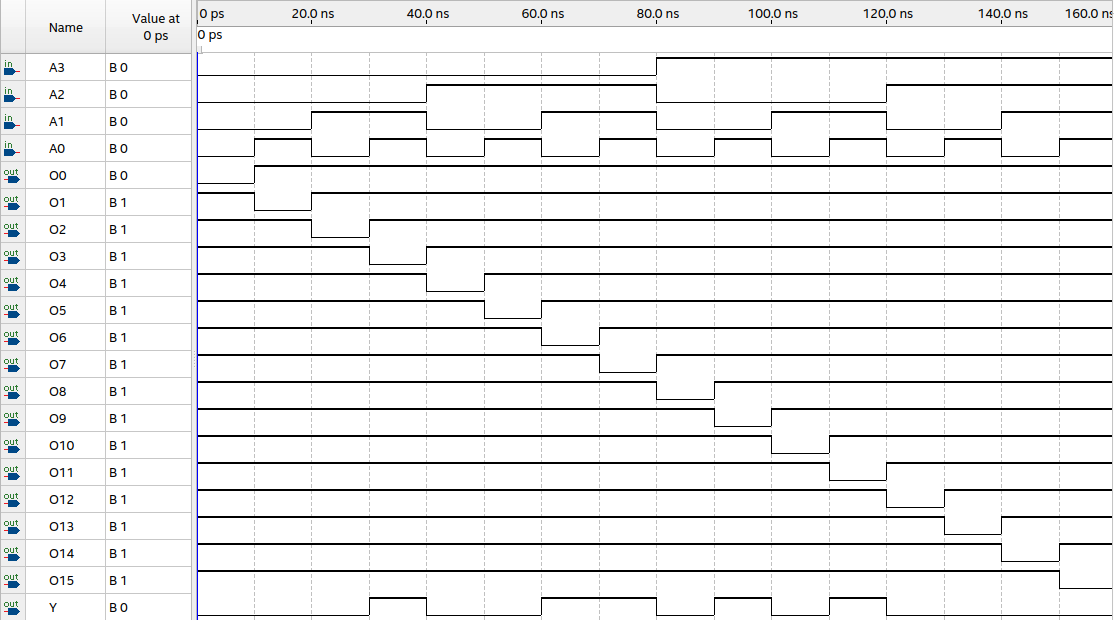
\includegraphics[width=\textwidth]{carta_tempos_dec.png}
  \caption{Carta dos tempos para o circuito construído com decodificadores}
  \label{fig:dec_sim}
\end{figure}

\begin{table}[!ht]
  \centering
  \caption{Tabela Verdade com valores esperados dos sinais de depuração $O_n$ e da saída final $Y$ para cada valor de entrada $A_m$ obtida a partir da Carta dos Tempos (Fig. \ref{fig:dec_sim}). Para redução de espaço, apenas os índices $n$ e $m$ dos sinais são mostrados no nome de cada coluna}
  \label{tab:dec_tb_verdade}
  \doubleRuleSep
  \begin{tabular}{*{21}{r}}
    \doubleTopRule
    \multicolumn{4}{c}{Entrada} & \multicolumn{16}{c}{Sinais de Depuração}                                                                                                                                                                                                                                                    \\
    \cmidrule(lr){1-4}\cmidrule(lr){5-20}
    $3$                         & $2$                                      & $1$        & $0$       & $0$      & $1$       & $2$        & $3$         & $4$       & $5$      & $6$       & $7$        & $8$         & $9$        & $10$      & $11$       & $12$        & $13$         & $14$       & $15$      & $Y$         \\
    \midrule
    \csvreader[head to column names, late after line=\\]{tb_verdade_dec_debug.csv}{}%
    {\csvcoli                   & \csvcolii                                & \csvcoliii & \csvcoliv & \csvcolv & \csvcolvi & \csvcolvii & \csvcolviii & \csvcolix & \csvcolx & \csvcolxi & \csvcolxii & \csvcolxiii & \csvcolxiv & \csvcolxv & \csvcolxvi & \csvcolxvii & \csvcolxviii & \csvcolxix & \csvcolxx & \csvcolxxi} %
    \doubleBottomRule
  \end{tabular}
\end{table}


\newpage
\subsubsection{Metodologia de montagem e de testes}
\label{sec:dec_montagem}

Durante a montagem, cada um dos decodificadores serão testados separadamente usando os oito leds da placa de montagem. A depuração será feita em duas etapas: a primiera metade ($A_3 = 0$) da Tabela \ref{tab:dec_tb_verdade} será testada conectando as saídas do decodificador C1 da Fig. \ref{fig:dec_diagrama} (sinais O0 a O7) nos leds da placa de montagem, e a segunda metade ($A_3 = 1$) da tabela será testada conectando as saídas do decodificador C2 (sinais O8 a O15) nos leds da placa de montagem.


\subsection{Circuito com Multiplexador} % R
\label{sec:mux}

\subsubsection{Diagrama lógico do circuito}
\label{sec:mux_diagrama}

Novamente, a partir da Tabela \ref{tab:tabela_verdade}, foi projetado um circuito digital mostrado no Diagrama Lógico da Figura \ref{fig:mux_diagrama} usando dois multiplexadores 74151 TTL, identificados por C1 e C2. As informações das entradas Vcc e Gnd dos componentes utilizados estão na Tabela \ref{tab:mux_entradas}.

O bit de entrada mais significativo foi conectado na porta enable do multiplexador C1 e invertido na porta enable do multiplexador C2.

Com isso, conseguimos utilizar o sinal de entrada de 4 bits a partir do cascateamento de dois multiplexadores 8x1, gerando, assim, um multiplexador 16x1.

\newpage

\begin{figure}[!ht]
  \centering
  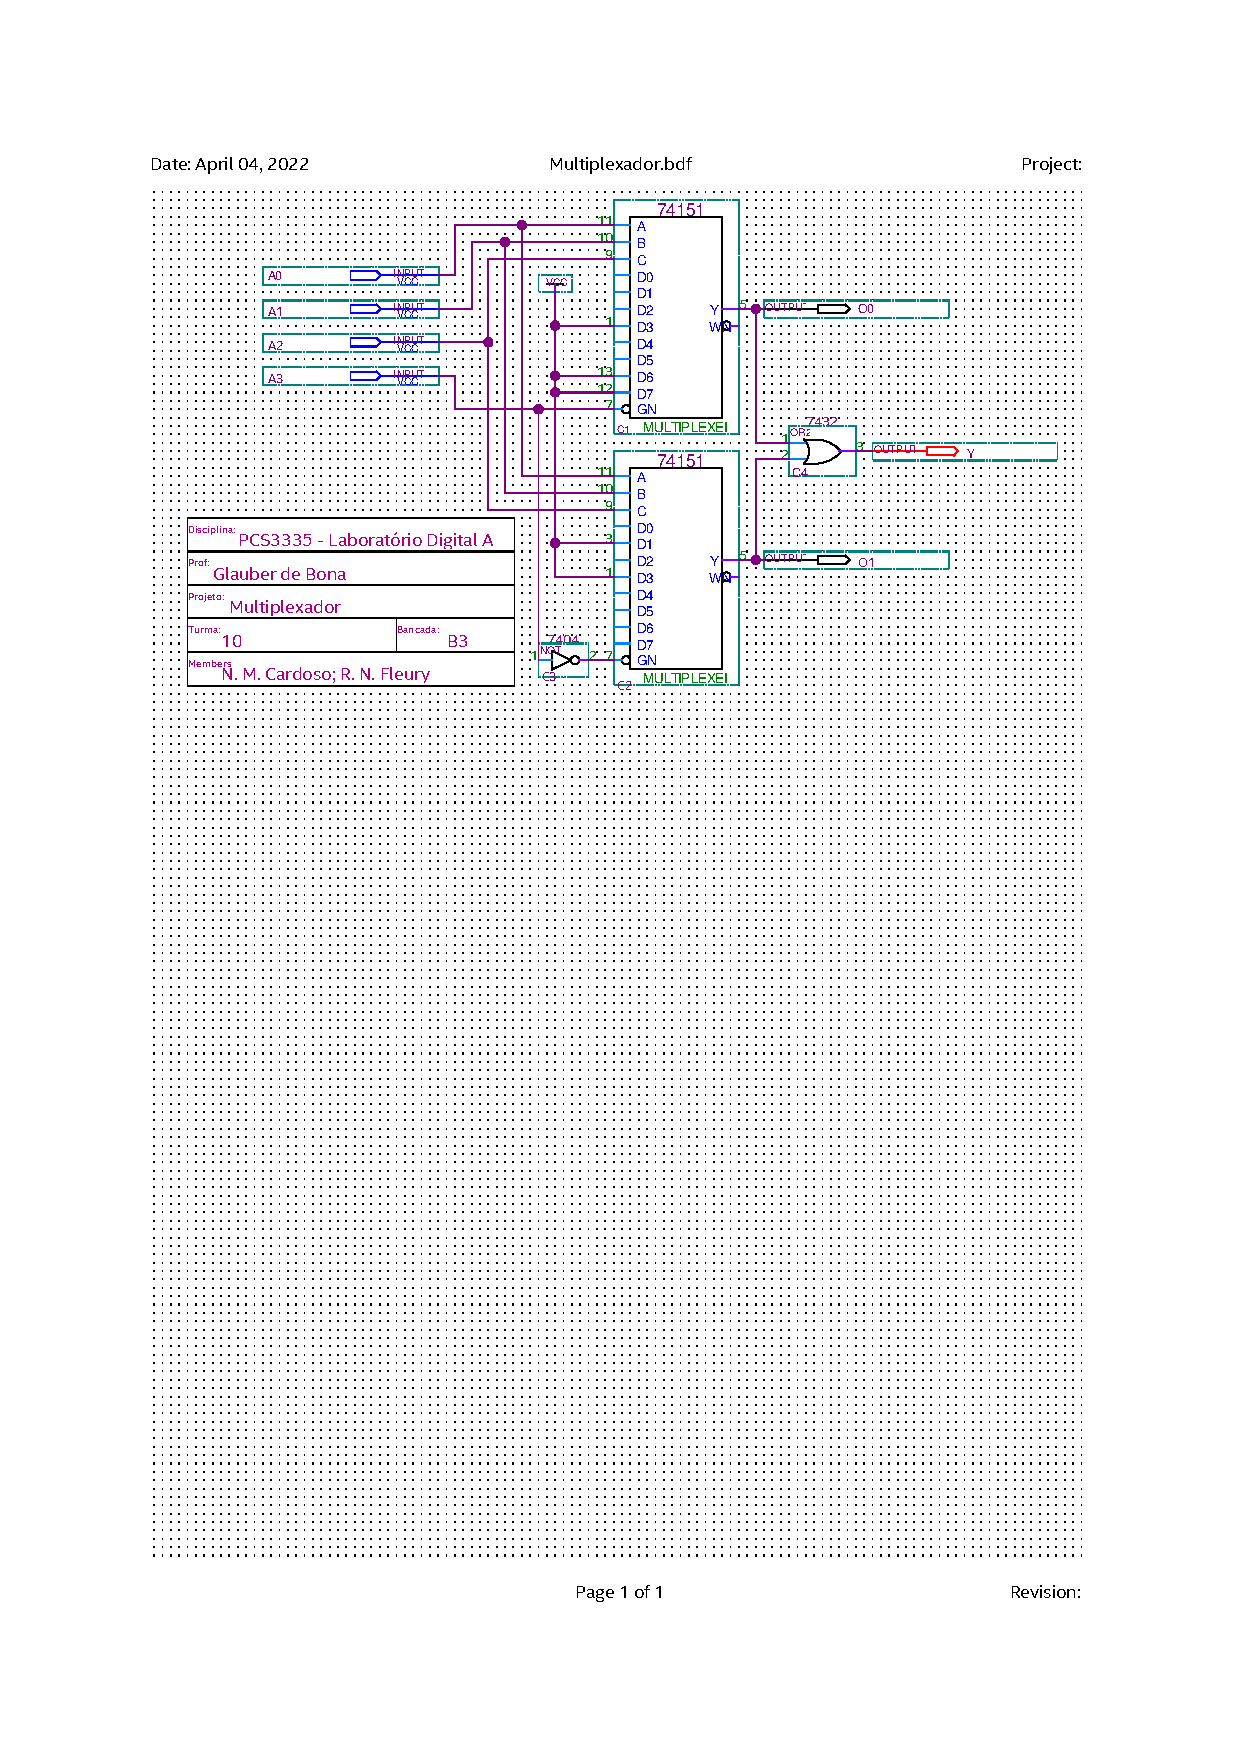
\includegraphics[width=\textwidth, trim={30mm, 179mm, 30mm, 30mm}, clip]{diagrama_mux.pdf}
  \caption[]{Diagrama lógico\footnotemark do circuito criado a partir da Tabela \ref{tab:tabela_verdade} com o uso de dois multiplexadores 74151 TTL.}
  \label{fig:mux_diagrama}
\end{figure}
\footnotetext{Imagem vetorial, é possível ampliar sem perder qualidade}

\begin{table}[!ht]
  \centering
  \caption{Informação das entradas Vcc e Gnd para cada componente identificado na Fig. \ref{fig:mux_diagrama}}
  \label{tab:mux_entradas}
  \doubleRuleSep
  \begin{tabular}{lrrr}
    \doubleTopRule
    Posição & Comp. & Vcc & Gnd \\
    \midrule
    C1      & 74151 & 16  & 8   \\
    C2      & 74151 & 16  & 8   \\
    C3      & 7404  & 14  & 7   \\
    C4      & 7432  & 14  & 7   \\
    \doubleBottomRule
  \end{tabular}
\end{table}

\subsubsection{Levantamento dos Materias Necessários}
\label{sec:mux_mat}

\begin{table}[!ht]
  \centering
  \caption{Unidades requeridas para cada CI}
  \label{tab:mux_materiais}
  \doubleRuleSep
  \begin{tabular}{lllrr}
    \doubleTopRule
    Slot & Operação & CI    & Un. Requeridas & Un. Disponíveis \\
    \midrule
    1    & MUX      & 74151 & -              & -               \\
    2    & MUX      & 74151 & -              & -               \\
    3    & NOT      & 7404  & 1              & 6               \\
    4    & OR       & 7432  & 1              & 4               \\
    \doubleBottomRule
  \end{tabular}
\end{table}

Para garantir que o circuito projetado respeite as restrições de montagem, fizemos um levantamento dos recursos necessários para este circuito mostrado na Tabela \ref{tab:mux_entradas}. Ela mostra a quantidade de unidades lógicas requeridas para cada CI utilizado. As especificações de cada CI foi obtido pelos respectivos \emph{datasheets}.

\subsubsection{Simulação}
\label{sec:mux_sim}

\begin{figure}[!ht]
  \centering
  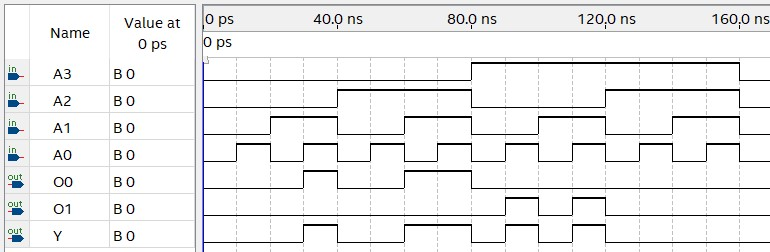
\includegraphics[width=\textwidth]{carta_tempos_mux.jpg}
  \caption{Carta dos tempos para o circuito construído com multiplexadores}
  \label{fig:mux_sim}
\end{figure}

\begin{table}[!ht]
  \centering
  \caption{Tabela Verdade com valores esperados dos sinais de depuração $O_0$ e $O_1$ e da saída final $Y$ para cada valor de entrada $A_i$ obtida a partir da Carta dos Tempos (Fig. \ref{fig:mux_sim}).}
  \label{tab:mux_tb_verdade}
  \doubleRuleSep
  \begin{tabular}{*{7}{r}}
    \doubleTopRule
    \multicolumn{4}{c}{Entrada} & \multicolumn{3}{c}{Depuração}                                                               \\
    \cmidrule(lr){1-4}\cmidrule(lr){5-7}
    $A_3$                       & $A_2$                         & $A_1$      & $A_0$     & $O_0$    & $O_1$     & $Y$         \\
    \midrule
    \csvreader[head to column names, late after line=\\]{tb_verdade_mux_debug.csv}{}%
    {\csvcoli                   & \csvcolii                     & \csvcoliii & \csvcoliv & \csvcolv & \csvcolvi & \csvcolvii} %
    \doubleBottomRule
  \end{tabular}
\end{table}

A carta dos tempos da simulação do circuito projetado (Fig. \ref{fig:mux_diagrama}) é mostrada na Fig. \ref{fig:mux_sim}. Além dos sinais de entrada A3, A2, A1 e A0 e do sinal de saída Y, inspecionamos os dois sinais imediatamente após os multiplexadores (O0 e O1) para a depuração. Com esta simulação concluímos que o circuito projetado possui a Tabela Verdade especificada na Tabela \ref{tab:tabela_verdade}. Assim, a Tabela \ref{tab:mux_tb_verdade} mostra a Tabela Verdade dos valores esperados para este circuito.

\subsubsection{Metodologia de montagem e de testes}
\label{sec:mux_montagem}

Durante a montagem, os dois multiplexadores serão testados ao mesmo tempo usando os sete primeiros leds da placa de montagem. A depuração será feita testando todas as possibilidades de entradas.



\section{Resultados}
Os sinais de depuração e de saída, obtidos durante e após a montagem do circuito, respectivamente, estão em conformidade com a Tabela Verdade dos valores esperados tanto para o decodificador (Tabela \ref{tab:dec_tb_verdade}) quanto para o multiplexador (Tabela \ref{tab:mux_tb_verdade}). Os valores experimentais dos sinais de saída para cada circuito estão dispostos na Tabela \ref{tab:tb_verdade_exp} do Apêndice \ref{ap:tb_verdade_exp}.

Para documentação, as Figs. \ref{fig:montagem1}, \ref{fig:montagem2} e \ref{fig:montagem3} do Apêndice \ref{ap:montagem} mostram a montagem final do circuito operando com diferentes valores de entrada.




\section{Conclusão}
Neste experimento, construímos circuitos combinatórios a partir de CI's com menor número de bits entrada usando a técnica de cascateamento de decodificadores e multiplexadores. Neste caso, usando dois decodificadores 3x8 para emular um 4x16 e dois multiplexadores 8x1 para emular um 16x1 usando o bit mais significativo como enable e invertendo em um dos CI's. Embora esta técnica seja intuitiva, é possível obter uma solução mais otimizada (usando menos componentes) a partir do método da Tabela Verdade Transformada para o multiplexador, conforme Seção 3.2.2 de \cite{saraiva}.

Durante a montagem do circuito, fizemos testes separados para cada CI combinatório. Logo no primeiro teste, verificamos que o sinal esperado não correspondia com o sinal obtido. Depois de diversos testes, notamos que duas das três portas do enable estavam operando em aberto. A descoberta tardia desta falha ocasionou no atraso da montagem do circuito. Então, para evitar este tipo de erro, nos próximos experimentos, representaremos, no diagrama lógico, um valor (Vcc ou Gnd) para portas de entrada não usadas ao invés de deixá-las em aberto, visto que a simulação funciona para ambos os casos e o circuito real não.

Por fim, os resultados obtidos experimentalmente estão em conformidade com os resultados planejados e não houve necessidade de alteração do planejamento durante o experimento.



\clearpage
\newpage
\appendix
\section*{Apêndice}
\renewcommand{\thesubsection}{\Alph{subsection}}

\subsection{Tabela Verdade experimental}
\label{ap:tb_verdade_exp}
\begin{table}[!ht]
  \centering
  \caption{Tabela Verdade dos circuitos construídos com decodificadores e multiplexadores apresentando os valores das saídas $Y_E$ (saída esperada), $Y_D$ (saída do decodificador) e $Y_M$ (saída do multiplexador) para cada entrada $A_3A_2A_1A_0$}
  \label{tab:tb_verdade_exp}
  \doubleRuleSep
  \begin{tabular}{rrrrrrr}
    \doubleTopRule
    \multicolumn{4}{c}{Entradas} & \multicolumn{3}{c}{Saídas}                                                               \\
    \cmidrule(lr){1-4}\cmidrule(lr){5-7}
    $A_3$                        & $A_2$                      & $A_1$      & $A_0$     & $Y_E$    & $Y_D$     & $Y_M$       \\
    \midrule
    \csvreader[head to column names, late after line=\\]{tb_verdade_exp.csv}{}%
    {\csvcoli                    & \csvcolii                  & \csvcoliii & \csvcoliv & \csvcolv & \csvcolvi & \csvcolvii} %
    \doubleBottomRule
  \end{tabular}
\end{table}

\newpage
\subsection{Montagem do circuito}
\label{ap:montagem}

\begin{figure}[!ht]
  \centering
  \begin{tabular}{cc}
    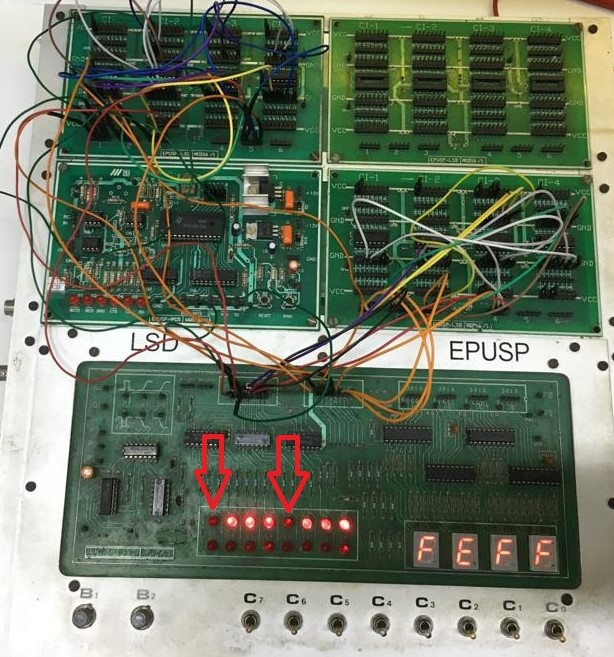
\includegraphics[height=0.49\textwidth]{0000_in.jpeg} & 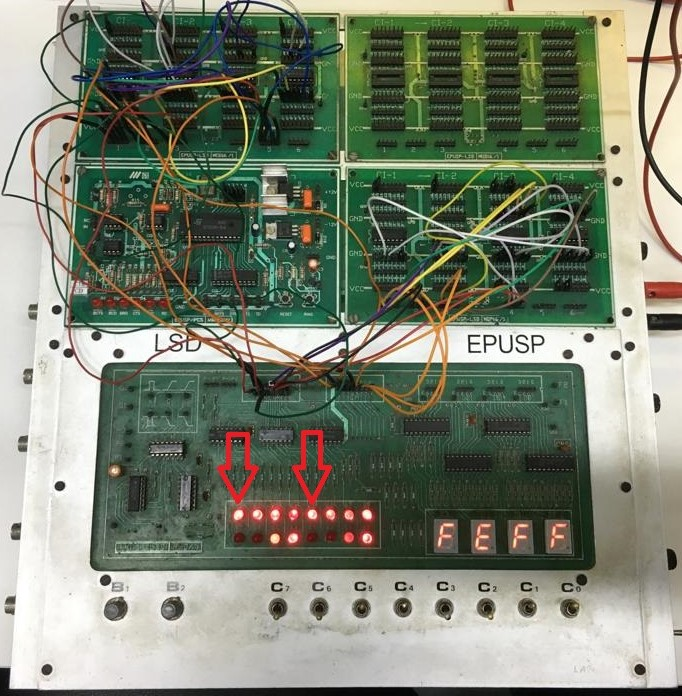
\includegraphics[height=0.49\textwidth]{0011_in.jpeg}
  \end{tabular}
  \caption{Montagem dos circuitos com o decodificador e o multiplexador simultanemente na mesma placa de montagem testando as entradas $0000$ (esquerda) e $0011$ (direita). Entradas do decodificador nas chaves de $C_7$ a $C_4$ e entradas do multiplexador nas chaves de $C_3$ a $C_0$ e saídas indicadas pela seta.}
  \label{fig:montagem1}
\end{figure}

\begin{figure}[!ht]
  \centering
  \begin{tabular}{cc}
    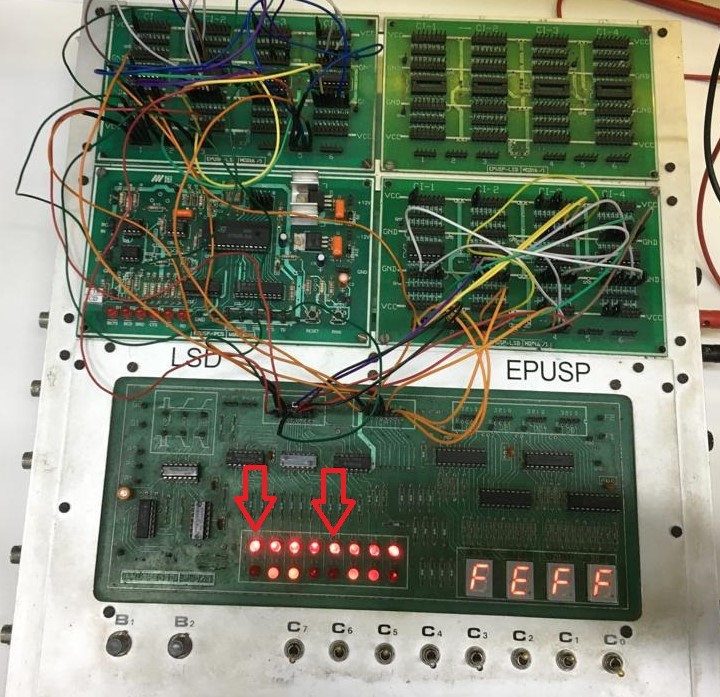
\includegraphics[height=0.47\textwidth]{0110_in.jpeg} & 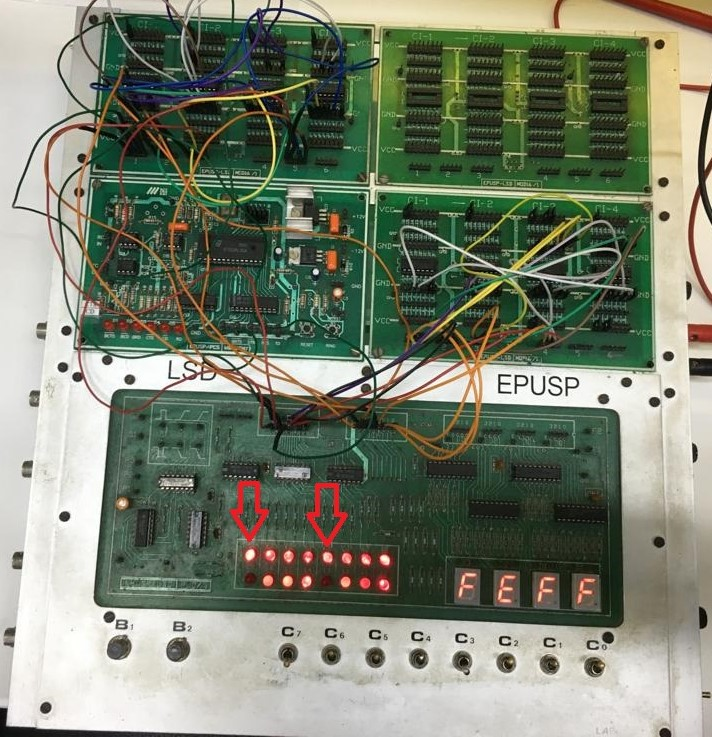
\includegraphics[height=0.47\textwidth]{0111_in.jpeg}
  \end{tabular}
  \caption{Montagem dos circuitos com o decodificador e o multiplexador simultanemente na mesma placa de montagem testando as entradas $0110$ (esquerda) e $0111$ (direita). Entradas do decodificador nas chaves de $C_7$ a $C_4$ e entradas do multiplexador nas chaves de $C_3$ a $C_0$ e saídas indicadas pela seta.}
  \label{fig:montagem2}
\end{figure}

\begin{figure}[!ht]
  \centering
  \begin{tabular}{cc}
    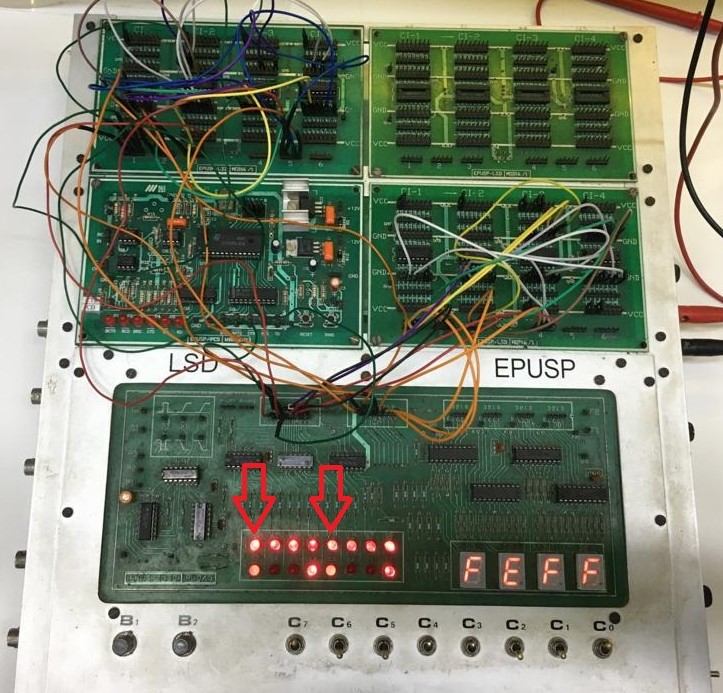
\includegraphics[height=0.46\textwidth]{1001_in.jpeg} & 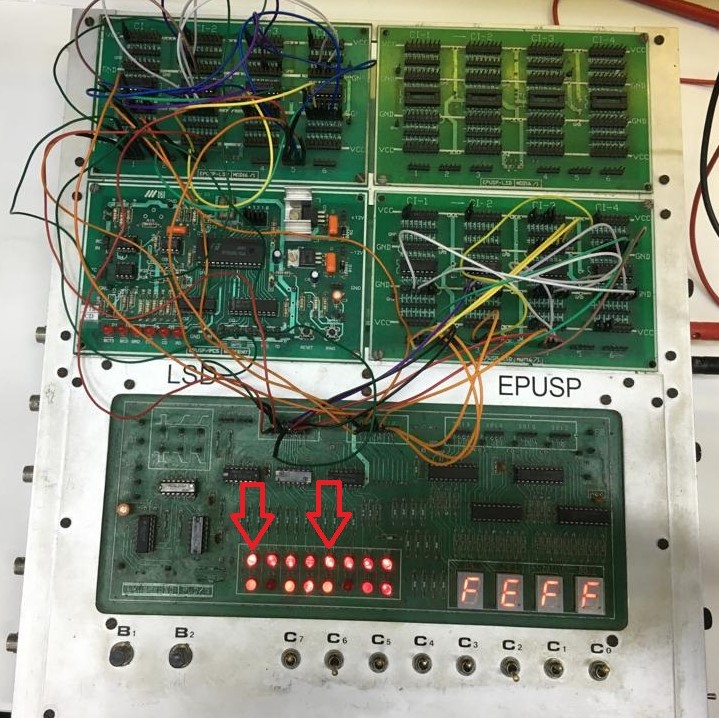
\includegraphics[height=0.46\textwidth]{1011_in.jpeg}
  \end{tabular}
  \caption{Montagem dos circuitos com o decodificador e o multiplexador simultanemente na mesma placa de montagem testando as entradas $1001$ (esquerda) e $1011$ (direita). Entradas do decodificador nas chaves de $C_7$ a $C_4$ e entradas do multiplexador nas chaves de $C_3$ a $C_0$ e saídas indicadas pela seta.}
  \label{fig:montagem3}
\end{figure}
\newpage

\bibliographystyle{unsrt}
\bibliography{refs}


\end{document}
